\documentclass[Dealing with Imbalance in Computer Vision]{IEEEtran}
\IEEEoverridecommandlockouts
% The preceding line is only needed to identify funding in the first footnote. If that is unneeded, please comment it out.
\usepackage{cite}
\usepackage{amsmath,amssymb,amsfonts}
\usepackage{algorithmic}
\usepackage{graphicx}
\usepackage{textcomp}
\usepackage{xcolor}
\def\BibTeX{{\rm B\kern-.05em{\sc i\kern-.025em b}\kern-.08em
    T\kern-.1667em\lower.7ex\hbox{E}\kern-.125emX}}
\begin{document}

\title{Dealing with Imbalance in Computer Vision\\
% {\footnotesize \textsuperscript{*}Note: Sub-titles are not captured in Xplore and
% should not be used}
\thanks{Identify applicable funding agency here. If none, delete this.}
}

\author{\IEEEauthorblockN{Mahir Pirmohammed,}
\IEEEauthorblockA{\textit{CSCE 421 Student} \\
\textit{Texas A\&M University,}
College Station, Texas \\
megamp15@tamu.edu}
% \and
% \IEEEauthorblockN{2\textsuperscript{nd} Given Name Surname}
% \IEEEauthorblockA{\textit{dept. name of organization (of Aff.)} \\
% \textit{name of organization (of Aff.)}\\
% City, Country \\
% email address or ORCID}
% \and
% \IEEEauthorblockN{3\textsuperscript{rd} Given Name Surname}
% \IEEEauthorblockA{\textit{dept. name of organization (of Aff.)} \\
% \textit{name of organization (of Aff.)}\\
% City, Country \\
% email address or ORCID}
% \and
% \IEEEauthorblockN{4\textsuperscript{th} Given Name Surname}
% \IEEEauthorblockA{\textit{dept. name of organization (of Aff.)} \\
% \textit{name of organization (of Aff.)}\\
% City, Country \\
% email address or ORCID}
% \and
% \IEEEauthorblockN{5\textsuperscript{th} Given Name Surname}
% \IEEEauthorblockA{\textit{dept. name of organization (of Aff.)} \\
% \textit{name of organization (of Aff.)}\\
% City, Country \\
% email address or ORCID}
% \and
% \IEEEauthorblockN{6\textsuperscript{th} Given Name Surname}
% \IEEEauthorblockA{\textit{dept. name of organization (of Aff.)} \\
% \textit{name of organization (of Aff.)}\\
% City, Country \\
% email address or ORCID}
}

\maketitle

\begin{abstract}
This article describes how to create a Convolutional Neural Network, Logisitc Regression, and Random Forest classifier on imbalanced training data that portrays the imbalanced data sets that are often acquired from real-world problems. The convolutional neural network  required many hidden layers to properly train on the different sections of the image and therefore did not need balanced data. The logistic regression and random forest were tuned using cross validation and stratified k fold to minimize the effect of the imbalanced data. Employing these techniques created high accuracies without changing the original data sets making them highly effective for other machine learning problems that use these imbalanced data.
\end{abstract}

\begin{IEEEkeywords}
Classifiers, Computer Vision, Digit Recognition, Imbalance, Machine Learning
\end{IEEEkeywords}

\section{Introduction}
Imbalance data occurs in many forms as the real world does not neatly provide data in a ready to use format. One of the most necessary skills in Machine Learning is  pre-processing or utilizing sampling techniques to minimize the effects of imbalanced data. Imbalanced data substantially compromises the learning process, since most of the standard machine learning algorithms expect balanced class distribution or an equal misclassification cost [1].  A common practice for dealing with imbalanced data sets is to rebalance them artificially. Doing so has been called "up-sampling"(replicating cases from the minority)   and "down-sampling" ignoring  cases  from  the  majority) [2]. In this article I reference up-sampling as over sampling and down-sampling as under sampling. To learn how to handle two common types of imbalanced data sets that simulate data from different real world scenarios: step imbalance and linear imbalance, I had to develop three classifiers: a convolutional neural network, random forest and logistic regression model.

The two imbalanced training data sets come from the MNIST data set which is a collection of 60,000 training and 10,000 testing Handwritten digit images commonly used to train and validate computer vision systems. In the data set each of the 0-9 digits is considered a class. In step imbalance as seen in ``Fig.~\ref{fig1}'' the data set has majority and minority classes where the amount of data in the majority and minority classes are approximately the same, but there is a large difference between majority and minority classes. On the other hand in linear imbalance data sets as seen in ``Fig.~\ref{fig2}'', the data has varying amounts of data in the different classes where one class can be very small and another very large.

\begin{figure}[]
\centerline{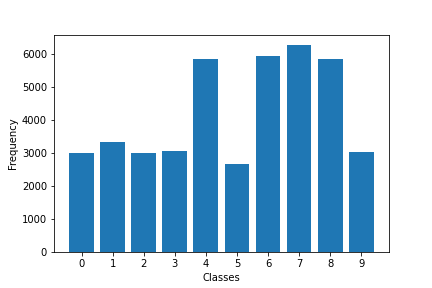
\includegraphics [width=200px]{dist step.png}}
\caption{Histogram of Step Imbalance.}
\label{fig1}
\end{figure}
\begin{figure}[]
\centerline{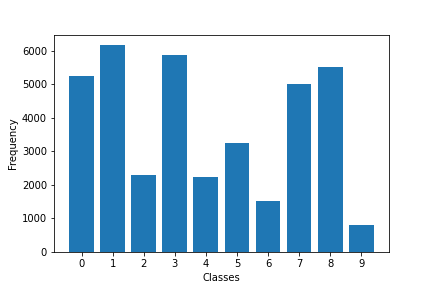
\includegraphics[width=200px]{dist linear.png}}
\caption{Histogram of Linear Imbalance.}
\label{fig2}
\end{figure}

\section{Methods Difference}
\subsection{Convolutional Neural Network (CNN) classifier}
Humans classify objects everyday through our repeated memories of the features of the objects and knowing their associated labels (names). The neural network is based on our brain's neurons which activate or deactivate based on certain conditions. These conditions can be attributed to features that a neural network can learn on and decide what are the most important to activate on to classify the different images. Convolutional Neural Networks are a special kind of multi-layer neural networks designed to recognize visual patterns directly from pixel images  with  minimal preprocessing [3].

The main architecture of a CNN consists of repeated convolusion layers, activation functions, spatial pooling (commonly downsampling), and fully connected layers. The convolusion layer extracts features of an image by merging the relationship of pixels next to each other depending on the number of output filters, the size of the filters (how much of the image does the filter look at), stride length (how much can the filters overlap as they slide over sections of the image), and padding (reduces the size of the image around the borders by adding 0's to the border) as seen in  in ``Fig.~\ref{fig3}''. The convolutional layer is accompanied by the activation function which activates certain features that are positive in each feature space in other words non-negative values to increase non-linearity between the pixels since images are naturally non-linear. The second most important architectural method in CNN's is spatial pooling or downsampling which reduces the dimensions of the input to make it more manageable without losing the important information. In our model we use max pooling which takes the many filters or features from the convolution layer and splits them into sections and the feature with the highest relevance or activation towards classifying the image is kept. This means that we can reduce the size of our feature space without losing important feature information about the image. The last layer in the CNN is the fully connected layer that learns the relationship between the many features that are outputted from the convolution layers. 
The CNN uses the Convolution layers, activation function and spatial pooling in forward propagation to calculate probabilities and errors 
from which the weights between neurons of each layer are updated using back propagation according to the amount of contribution that filter or feature had to the total error. 
In my implementation of a CNN, I use a 7 layer model proposed in [3] that has layers in the following order: 
\begin{enumerate}
    \item Convolution with a Rectified Linear Unit (ReLU) Activation Function that creates an activated feature map of size 24*24 of 32 filters of size 5*5 with a stride input of one and zero padding. 
    \item A max pooling layer has a size of 2 with a stride of 2 to reduce the 32 feature map size by half to 12*12.
    \item A second convolution layer with a (ReLU) activation function that extracts 32 filters from the reduced 12*12 input with the same hyper-parameters of size, stride, and padding to get an activated feature space of size 8*8 of 32 filters. 
    \item The second max pooling takes place with the same hyper-parameters of size and stride to reduce our feature map to a size of 4*4 of 32 filters.
    \item We finally get to a fully connected layer which uses a convolution operation to create 64 filters of dimension 1*1.
    \item We repeat the previous layer using a convolution operation to get an output of 256 filters of dimension 1*1 which includes the (ReLU) activation function.
    \item Now with the activated fully activated layer we use softmax to get probabilities of the 256 filters being in a specific class of the 10 digits.
\end{enumerate}

The convolutional neural network is trained in batches of images which calculate a loss per batch that is used by the stochastic gradient descent optimizer in back propagation. In back propagation the optimizer updates the weights between the neurons that are used by the Rectified Linear Unit (ReLU) activation function to activate or deactivate neurons based on there contribution to the total error in order to minimize the loss in future batches.  

This is how I implemented the CNN model to work against the imbalanced data sets and still get high accuracy scores. By having 7 layers that broke down the most important features of each image into 256 filters that were then used to compute the class probabilities, small batch sizes that enabled the weights to be updated by back propagation many times, and repeating this for many epochs to ensure each class has enough data and filters to properly classify the test data.

\begin{figure}[]
\centerline{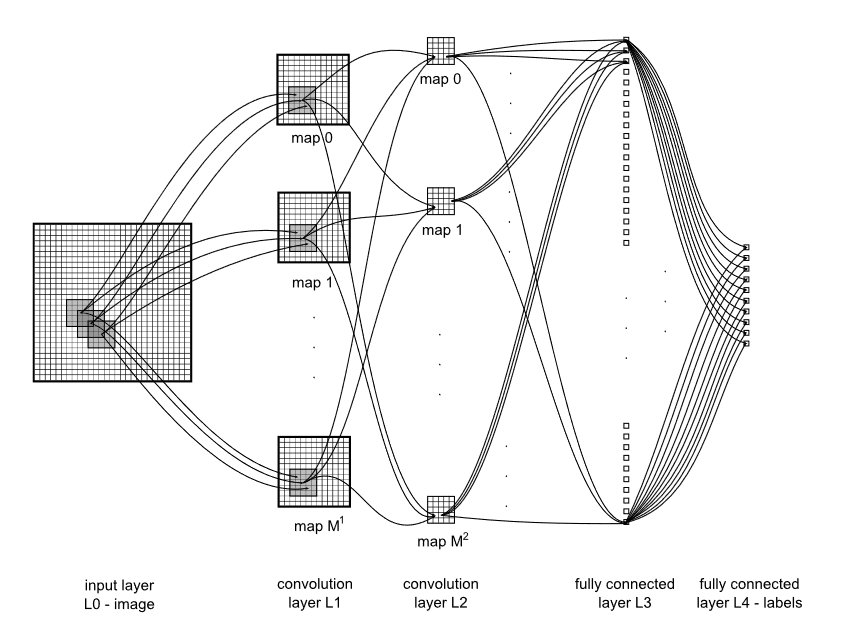
\includegraphics[width=275px]{layers.PNG}}
\caption{Architecture of a convolutional neural network withfully connected layers, kernel sizes of 5 x 5 and skipping factors of 1 [4].}
\label{fig3}
\end{figure}

\subsection{Logistic Regression Classifier}
Logistic Regression is a model that uses the logit function or a sigmoid to predict the probabilities of a class between 0 and 1 based on the weights associated with each feature. In my implementation I used the limited memory BFGS solver which is an optimization algorithm in the Newton Method family that performs gradient descent and hessian of the logistic cost function because of the limited amount of computer memory I had and the faster training time. We use the results from the solver to iterate against the negative direction of the gradient with some alpha learning rate until we reach convergence.

Other things I implemented in my logistic regression classifier was stratifying the two different imbalanced data sets into 10 different groups that each had the same class proportions as the original data. Along with this I did a 5 fold cross validation using sklearn's GridSearchCV which enabled me to see what was the best c hyperparamter for the data. The c hyperparameter is the inverse of the regularization strength. Regularization strength is the amount of penalty on features to reduce over-fitting since the training phase will try to fit exactly to the training data. By having a smaller c value, the regularization strength is increased which increases the chance of predicting correctly on unseen data. By choosing a range of c values for GridSearchCV, I was able to better determine the proper hyperparameter to overcome the training imbalance of the step and linear data set by having a large regularization strength. Also by splitting the 10 groups into 3 more cross validation sub groups, I had created 50 subgroups that would be trained on the model to improve the weights and compute the gradient differences many times. This minimized the effect of the classifier from being over trained on the majority classes in the data set and being able to train the minority classes between the different sub groups. I also used over and under random sampling to see if leveling the amount of data in each class would improve the accuracy of the model because machine learning models assume that they are being fed balanced data.

\subsection{Random Forest Classifier}
Random Forest is a collection of ensemble method (divide-and-conquer approach) decision trees with short depths that are generated on the randomly split data set. Decision trees create there different branches according to information gain or gini index on the input data provided. The gini index is a sum of the squared proportions of each class in the input data and this decides the big decision splits in a binary format using the knowledge of the variance of the input data set. Information gain is the concept that more information reduces uncertainty and uses entropy as the measure of uncertainty. Entropy for discrete distributions is the average inverse proportion of its probability. For continuous distributions the entropy depends on the variance of the data and for conditional entropy it depends on the probability of the outcome from a set of features or attributes. The branches are created with the features or attributes with the most information gain or least entropy from all the possible attribute outcomes from the parent to child branch. Then in the prediction phase the model inputs each image from the test data into all the individual random decision trees to decide on the leaf or class that image should belong to using a majority vote. 

In my implementation of the random forest classifier, I used a similar approach to the logistic regression model by using 10 stratified k folds and an inner 5 fold cross validation using GridSearchCV on a range of hyper-parameters for the number of trees and max depth from Sklearn. This enabled me to have 50 subgroups that would be fed into the random forest classifier to create even more randomly generated decision trees so the model can better train on the input data. 
This method of sampling the original data into smaller sub groups of evenly distribution proportions to the original data set and then randomly separated into small decision trees enabled the model as a whole to over come the imbalanced training data. I also used the over and under random sampled training data in the random forest implementation to see if a balanced data set would improve the accuracy of my model because in addition to the machine learning model now having fed balanced data, the edge cases for the minority classes can be covered the same amount of times as the majority classes.

\section{Test Results}
\subsection{Metrics}
The evaluation criteria is a key factor in assessing the classification performance and guiding the classifier modeling [5]. From a classification matrix we can compute 4 metrics as shown in [4]:
\begin{enumerate}
    \item True positive rate is the percentage of positive instances correctly classified.
    \item True negative rate is the percentage of negative instances correctly classified.
    \item False positive rate is the percentage of negative instances misclassified.
    \item False negative rate is the percentage of positive instances misclassified. 
\end{enumerate}

These 4 metrics on there own do not quantify the quality of our models. One measure that can result from this is the Receiver Operating Characteristic (ROC). This allows the visualization of the trade-off between the benefits (True Positive Rate) and costs (False Positive Rates), as it evidences that any classifier cannot increase the number of true positives without also increasing the false positives [5]. Using this ROC metric we can create an area under the curve graph that shows the average performance of the model (AUC-ROC). The closer the area is to one the closer the model is to correctly classifying a prediction as seen in ``Fig.~\ref{fig4}''.

\begin{figure}[]
\centerline{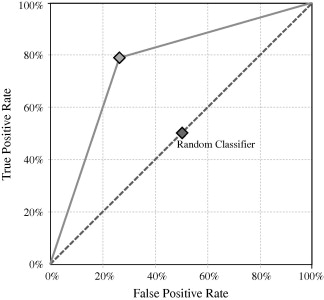
\includegraphics[width=200px]{AUC_ROC.jpg}}
\caption{An area under the Receiving Operating Characteristic Curve that shows a solid line classifier is better than the dashed line random classifier [5]. The closer to the upper left corner, the closer the area is to 1.}
\label{fig4}
\end{figure}

\subsection{Convolutional Neural Network Classifier Results}
\begin{itemize}
  \item The AUC ROC Scores for Imbalanced Linear: 0.99164
  \item The AUC ROC Scores for Over-sampled Linear: 0.98028
  \item The AUC ROC Scores for Imbalanced Step: 0.99217
  \item The AUC ROC Scores for Over-sampled Step: 0.98651
\end{itemize}

The AUC ROC metric defined above shows us that the implementations discussed work effectively to classify the test images into the 10 digit classes with scores close to 1. Using the over-sampled data set reduced the accuracy of our model because of over-fitting to the training data set. In the confusion matrix in ``Fig.~\ref{fig5}'', we can see that the most misclassification occured for class 9 with a max misclassification of 110 images. We can see the reason that class 4 was predicted for class 9 is due to more data present for class 4 than class 9 in the step imbalanced data set as seen in ``Fig.~\ref{fig1}''.

\subsection{Logistic Regression Classifier Results}
All models chose a c value of 0.01.
\begin{itemize}
    \item The AUC ROC scores for Imbalanced Linear: 0.99282
    \item The AUC ROC scores for Over-sampled Linear: 0.99282
    \item The AUC ROC scores for Under-sampled Linear: 0.99251
    \item The AUC ROC scores for Imbalanced Step: 0.99294
    \item The AUC ROC scores for Over-sampled Step: 0.99301
    \item The AUC ROC scores for Under-sampled Step: 0.99286
\end{itemize}

The AUC ROC metric for Logistic Regression is similar if not higher than the score for CNN but it still does well to classify the test data as seen in ``Fig.~\ref{fig6}''. The over/under sampled data sets did not seem to improve or decrease the accuracy of our model by a significant margin. The Step training data sets improve our accuracy over the linear training step slightly when testing on the test data set. In the confusion matrix in ``Fig.~\ref{fig6}'', we see that the misclassification values are smaller for each class and the max is only 50 compared to CNN's max misclassification value which improved our AUC ROC score slightly.

\subsection{Random Forest Classifier Results} 
All models chose a max depth of 10 from a range of 1 to 10.
All models chose the max number of trees of 150 from a range of 10 to 150.
\begin{itemize}
    \item The AUC ROC scores for Imbalanced Linear: 0.996499
    \item The AUC ROC scores for Over-sampled Linear: 0.996925
    \item The AUC ROC scores for Under-sampled Linear: 0.996392
    \item The AUC ROC scores for Imbalanced Step: 0.997190
    \item The AUC ROC scores for Over-sampled Step: 0.997352
    \item The AUC ROC scores for Under-sampled Step: 0.997262
\end{itemize}
The AUC ROC metric for Random Forest did the best out of the three. The Step training data sets improve our accuracy over the linear training slightly when testing on the test data set. In the confusion matrix in ``Fig.~\ref{fig7}'', we see that the max misclassification value increased to 57 again for class 9 and class 4 but misclassification overall decreased with many 0's appearing. This increased our AUC ROC score 0.04 and 0.05 over Logistic Regression and CNN respectively.
\begin{figure}[]
\centerline{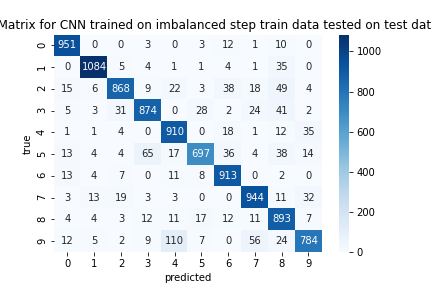
\includegraphics[width=200px]{Confusion_Matrix_CNN_trained_imbalanced_step_train.png}}
\caption{Confusion Matrix for CNN trained on imbalanced step data set with the highest ROC AUC score of 0.99217.}
\label{fig5}
\end{figure}

\begin{figure}[]
\centerline{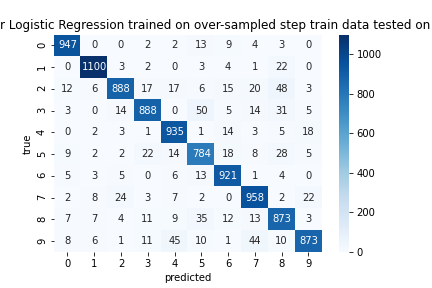
\includegraphics[width=200px]{Confusion_Matrix_Logistic Regression_trained_over-sampled_step_train.png}}
\caption{Confusion Matrix for Logistic Regression classifier trained on over sampled step data set with the highest ROC AUC score of 0.99301.}
\label{fig6}
\end{figure}

\begin{figure}[]
\centerline{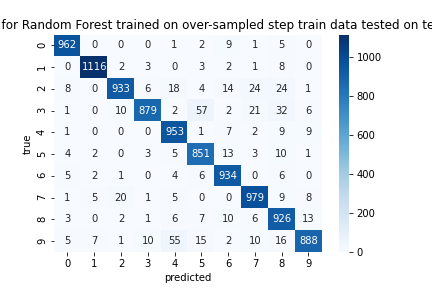
\includegraphics[width=200px]{Confusion_Matrix_Random Forest_trained_over-sampled_step_train.png}}
\caption{Confusion Matrix for Random Forest trained on over sampled step data set with the highest ROC AUC score of 0.997352.}
\label{fig7}
\end{figure}

\section{Comparison of Techniques}
The results show that CNN with its 7 layers architecture did the worst at classifying the test data with its best AUC ROC score around the linear regression AUC ROC score. This is because while decreasing the complexity of the feature map using max pooling but increasing the amount of filters we are letting the network train on layer by layer, resulting in 256 filters per image. This in combination with the many epochs that the CNN is trained through, the majority classes have even more data in comparison to the minority classes. This would cause the neurons to deactivate certain features the minority classes would need since there is more majority class data to re-weight the weights in between the layers that is used for activation. This is what causes over-fitting to the training data especially when using sampling data sets. As said in [4] for under sampling, the major drawback is that it can discard potentially useful data, that could be important for the learning process. For random oversampling, several authors agree that this method can increase the likelihood of occurring over-fitting, since it makes exact copies of existing instances [5]. We see this in the AUC ROC score of the over-sampled trained CNN models as they drop by approximately 0.05 to 0.1. 

The Logistic Regression classifier in contrast did the second best out of the three classifiers. This is because of the high regularization strength because of a small c value of .01 that was chosen due to a high 1e8 high convergence limit. With these optimal values the logistic regression algorithm was able to generalize a little bit better than CNN but it struggled to classify the same minority classes as CNN. The score was higher especially on the over-sampled step training data set. The increase in data values for the majority classes enabled the logistic regression algorithm to decrease the misclassifications between the minority and majority classes as we saw with the decrease of max misclassifications to 50. This improved the score of AUC ROC over CNN by .001.

The random forest classifier scored highest in the area under the receiver operating characteristic curve (AUC ROC) than logistic regression and convolutional neural network. Since the random forest optimally chooses to increase the number of decision trees and decrease the depths of the trees as well as randomize the input data sets by randomly splitting the original data set, we get many short decision trees where many may have more minority class samples than majority. With this model along with the stratified k fold and 5 fold cross validation sub groups I used in the implementation created a higher chance of creating many minority decision trees which improved the classification of minority digits and increased AUC ROC. The model chose 150 decision trees of max depth 10 because of the large amount of data present.  If more resources were available then the number of trees can be boosted to a higher number to have a higher change of having more decision trees with the minority classes so that the AUC ROC could be closer to 1.

\section{Conclusion}
Through the creation of three different classifiers, I explored two common variations of imbalanced data sets representing different real-world scenarios: step and linear. I discovered that imbalanced data sets affect the model greatly and countermeasures such as preprocessing and sampling need to be utilized to improve the underlying algorithms of each model. By using normalization, over-sampling, under-sampling, stratified k fold, and k fold cross validation with GridSearchCV from sklearn to find the best hyperparameters for the different data sets, I was able to create a convolutional neural network, a logistic regression classifier, and random forest classifier with above .99 AUC ROC scores. Although there is room for improvement as misclassification can be costly when it comes to the context of the data set such as classifying tumors in patients, this was a great first step at understanding the underlying algorithms of machine learning models in order to counteract common classification problems that occur in the real world such as imbalanced data. Going forward I will use more computer resources and time to find the optimal hyper-parameters by adding more parameters, and increasing the number of stratified k folds for the Logistic Regression and Random Forest Classifiers. For CNN I shall experiment with more or less layers, increase or decrease learning rate, changing the batch size of the training loop, and the amount of epochs to improve the classification of each class without over-fitting to the training data.

\begin{thebibliography}{00}
\bibitem{b1} G. Lemaitre, F. Noguiera, and C. K. Aridas, ``Imbalanced-learn: A Python Toolbox to tackle the Curse of Imbalanced Datasets in Machine Learning,'' \emph{The Journal of Machine Learning Research}, vol. 18, no. 1, pp. 1, Jan. 2017.
\bibitem{b2} F. Provost, ``Machine Learning from Imbalanced Data Sets 101,'' AAAI, Rep. WS-00-05, 2000.
\bibitem{b3} Md. A. Hossain and Md. M. Ali, ``Recognition of Handwritten Digit using Convolutional Neural Network,'' Global Journals, vol. 19, no. 2, pp. 1-5, 2019
\bibitem{b4} D. C. Ciresan, U. Meier, J. Masci, L. M. Gambardella, and J. Schmidhuber, ``Flexible, High Performance Convolutional Neural Networks for Image Classification,'' presented at the Twenty-Second International Joint Conference on Artificial Intelligence, Barcelona, Spain, July 16-22, 2011
\bibitem{b5} V. Lopez, A. Fernandez, S. Garcia, V. Palade, and F. Herrera, ``An insight into classification with imbalanced data: Empirical results and current trends on using data intrinsic characteristics,'' Information Sciences, vol. 250, no. 20, pp. 113-141, Nov. 2013, doi: 10.1016/j.ins.2013.07.007.

\end{thebibliography}
\vspace{12pt}

\end{document}
